\chapter{用户与微软账号}
\label{cha:user-and-ms-account}

\begin{intro}
  本章我们介绍 Windows 系统中的「用户」概念,以及微软账号的相关事项。看完本章,你或许可以找到这些问题的答案:

  \begin{itemize}
    \item 为什么我自己的电脑还有「用户」?
    \item 什么是微软账号(Microsoft 账户\footnotemark)?我为什么被要求注册/登录微软账号?
    \item 在\chapref{cha:basic-maintenance}中提到的「UAC 弹窗」和「以管理员身份运行」究竟是什么?
    \item 谁是「系统管理员」?
    \item 登录微软账号有什么好处?
    \item 要是我想改掉自己用户文件夹的名称该怎么做?
  \end{itemize}
\end{intro}
\footnotetext{注意,由于微软的疏忽,Windows 中多用「帐户」一词,然而正确的写法应是「账户」,但本文为忠于原文,未更改相关词汇。}

「用户」的概念是现代计算机操作系统的一个重要组成部分。尽管在今天,绝大多数电脑都仅为个人使用,「多用户」的理念似乎正渐渐模糊,但我们依然有必要了解这套机制的运作过程。

\section{「用户」概念的产生}

三十年前,电脑对于人们来说还是可望而不可得的「奢侈品」。当时,只有在少数学校和科研院所,才能看到数量有限的电脑。在这样的情况下,自然免不了多人共用一台电脑来学习和工作。为了隔离每个人在电脑上保存的文件和偏好设置,「用户」这个概念便应运而生。

如同 QQ 之类的社交软件一样,在有「用户」概念的系统中,我们可以在一台电脑上建立一个或者多个「用户」。在每次开机启动时,我们可以在用户列表中选择合适的身份来「登录」(\autoref{fig:Choose_User_when_Login} 左下角,图中选择的用户是「Windy」)。

\begin{figure}[htb!]
  \centering
  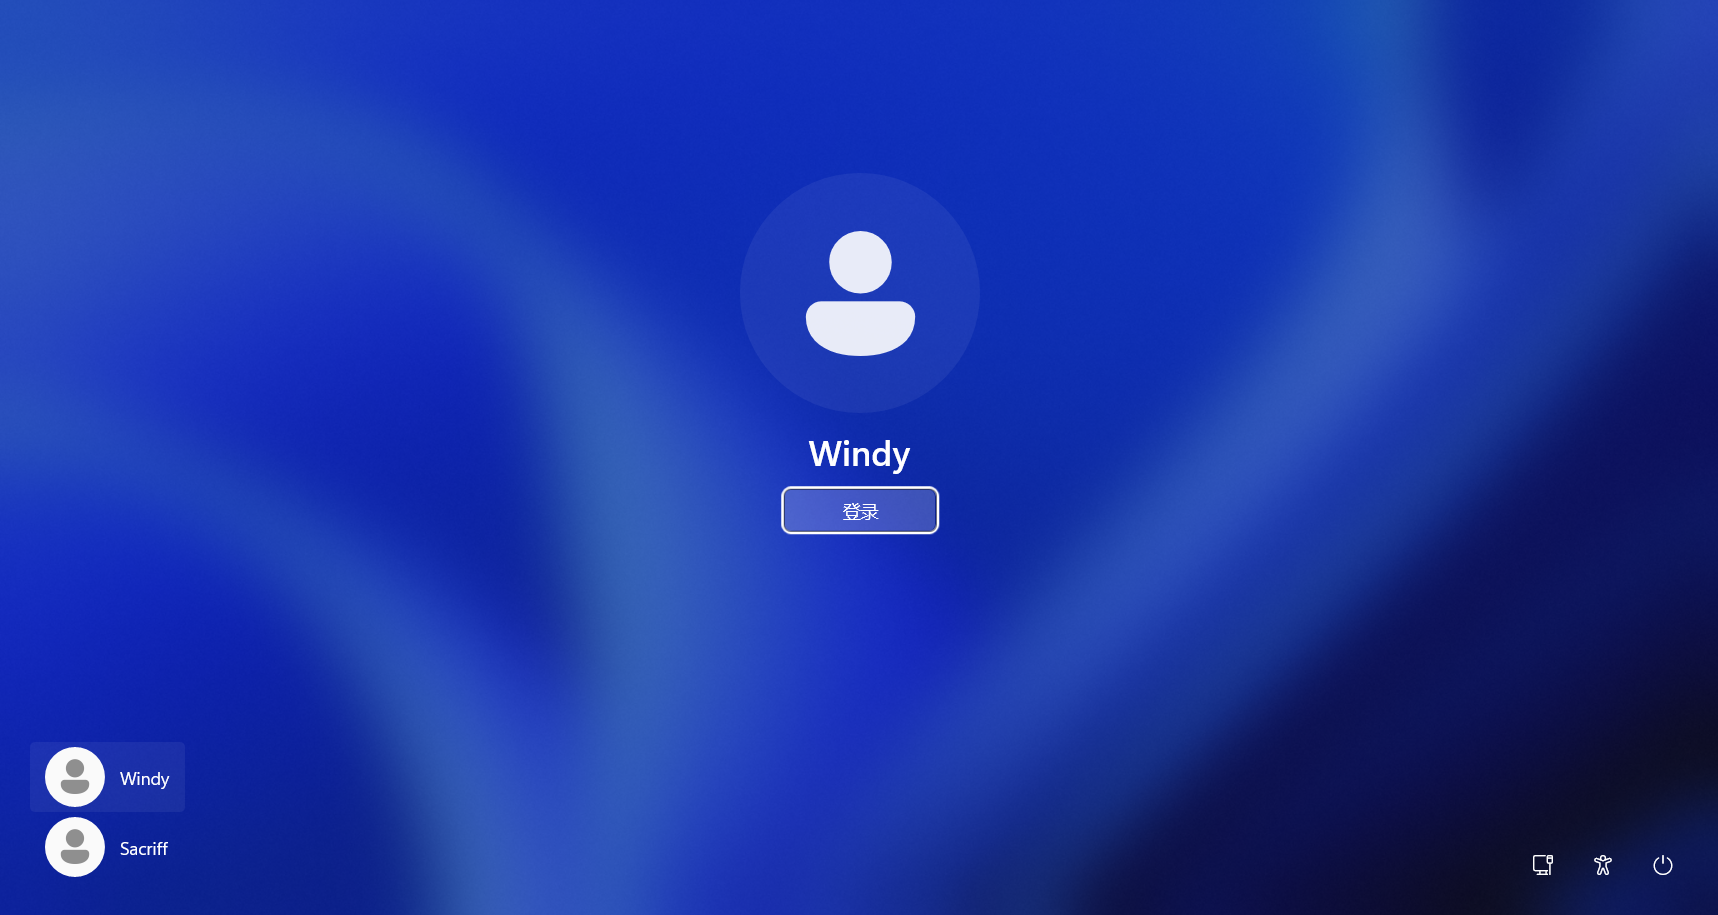
\includegraphics[width=.7\textwidth]{assets/advanced/Choose_User_when_Login.png}
  \caption{Windows 11 的登录界面}
  \label{fig:Choose_User_when_Login}
\end{figure}

在这样的系统中,每个用户拥有自己独立的用户名和密码,且每个用户在自己的「用户配置文件夹」(俗称「用户文件夹」,参见\chapref{cha:file-and-file-management})内保存的文件,其他用户均无法看到。每个用户设置的桌面壁纸、颜色风格等都互不影响。在多用户系统的加持下,人们成功实现了「一台电脑,多人在不同时段共用」这一目标。

时过境迁,电脑逐渐普及,成为了每个人工作和生活的必需品,那种「多人不得不共用一台电脑」的日子也渐渐成为历史\footnote{不过,在学校、企业、科研机构等场所,「多人共用一台高性能电脑」的情况仍然非常普遍。这种高性能的电脑通常被称为「服务器」,一般保持 24 小时运行,人们通过「远程连接」的方式来使用它们。服务器既有运行 Windows 系统的,也有运行 Linux 系统的,视人们的需求而定。}。然而,「多用户」这一思想却一直流传下来,形成了今天电脑系统的标配。尽管今天的个人电脑大都真的只是「个人」电脑——由一个人使用,多用户系统依然在我们的系统中得以保留,并在权限控制等特殊方面起着非常重要的作用。

\section{Windows 系统中的「用户」}

在我们第一次启动 Windows 系统(参见\chapref{cha:new-laptop-setup}))时,系统会要求设置一对用户名和密码,这其实就是在创建我们自己的用户\footnote{如果你在第一次开机时直接登录了微软账号,那么系统会先用你的微软账号的前 5 位作为用户名新建一个「本地帐户」\CJKsout*{,然后你就会发现一个巨难看的本地用户名},然后迅速将它连接到你的微软账号(参见后文)。整个过程对你来说完全无感。}。打开 \MissingVerb{C:\用户\} 目录,你可以看到一个以它命名的文件夹,以及一个 \MissingVerb{公用} 文件夹:

\begin{figure}[htb!]
  \centering
  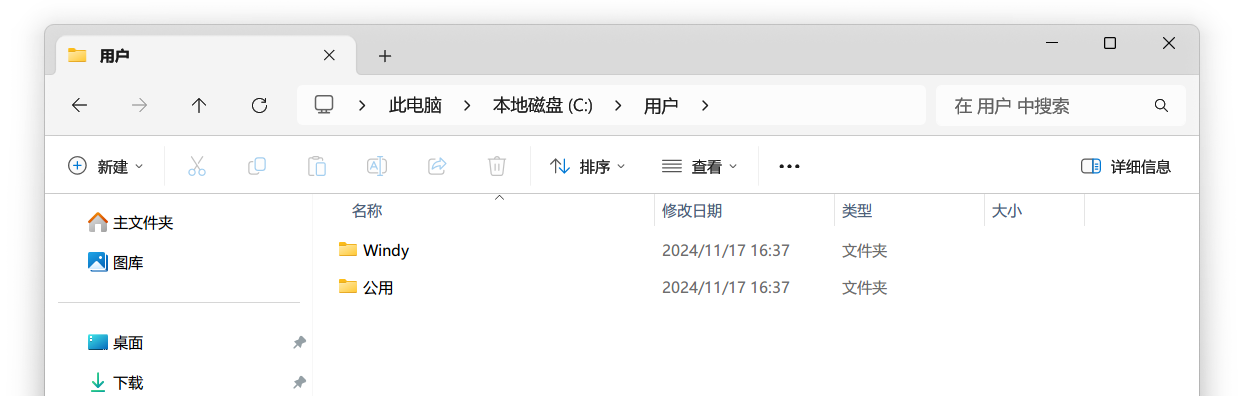
\includegraphics[width=.8\textwidth]{assets/advanced/C_Users_folder.png}
  \caption{用户文件夹}
  \label{fig:C_Users_folder}
\end{figure}

在那个与你的用户名同名的文件夹中,放置着你的用户文件和诸如「文档」「下载」等已知文件夹(如果你没有按照\chapref{cha:file-and-file-management}中介绍的过程去迁移它们的话)。可以想象,假如这台电脑上还有另外的几个用户,那么在 \MissingVerb{C:\用户\} 将罗列着多个用户的文件夹。每个用户都只能打开属于自己的那个文件夹以及 \MissingVerb{公用} 文件夹,从而实现了「多个用户资料的隔离」与「用户间资料的共享」。

在前文我们已经讲过,「文档」「下载」这样的已知文件夹是微软好心留给我们,帮助我们整理文件的。现在你应该能理解这样的好心了:Windows 本身就是一个为多用户设计的系统,从其他用户的角度考虑,用户的文件只有放在 \MissingVerb{C:\用户\<用户名>\} 这里才比较安稳——至于什么「这里是 C 盘,不适合放文件」,那微软才不管呢。

\section{用户与权限,以及 Administrator}

上文有说,今天保留多用户机制的一个很重要的原因,就是它能够更好地实现系统权限的分离。还记得\chapref{cha:basic-maintenance}中提到的权限相关的知识吗?在这里,我们会更深入地探讨这个话题。

大多数时候,我们会接触到两层权限——「标准用户权限」和「管理员权限」,顾名思义,后者的权限肯定高出不少。仅凭标准用户权限,我们无法直接在 C 盘写入文件,不能往 C 盘的全局软件目录里安装、卸载软件,更不可更改系统关键设置……这些都是需要管理员权限才能做的事情。

在 Windows 中,我们可以创建的用户也有两种——「标准用户」和「管理员」。显然,标准用户只有一层标准用户权限,但与直觉上可能相悖的一点是:\regcolor{管理员可以在标准用户权限和管理员权限两层之间切换。}同时,\regcolor{管理员在正常使用电脑时,也处在标准用户权限的层级下。}我们直接打开一个程序时,由于处在标准用户权限的范围内,程序也只能获得标准的权限。

\begin{note}
  我们在第一次开机时创建的那个用户一定是管理员,毕竟系统没个管理员显然是不行的。
\end{note}

与标准用户不同,Windows 为管理员提供了一套「提升权限」的机制:在\chapref{cha:basic-maintenance} 中,我们说「右击一个程序选择【以管理员身份运行】,就可以赋予程序提升的权限」,这一操作的实质,就是我们将自己的权限层级临时提升至管理员权限。那个「UAC 弹窗」的本质,就是某个程序试图让我们提升权限来执行它自己时,Windows 系统弹出的警告。一旦选择【是】,我们的权限就临时变更为管理员层级,而对应的程序亦借此有了管理员权限。

\begin{figure}[htb!]
  \centering
  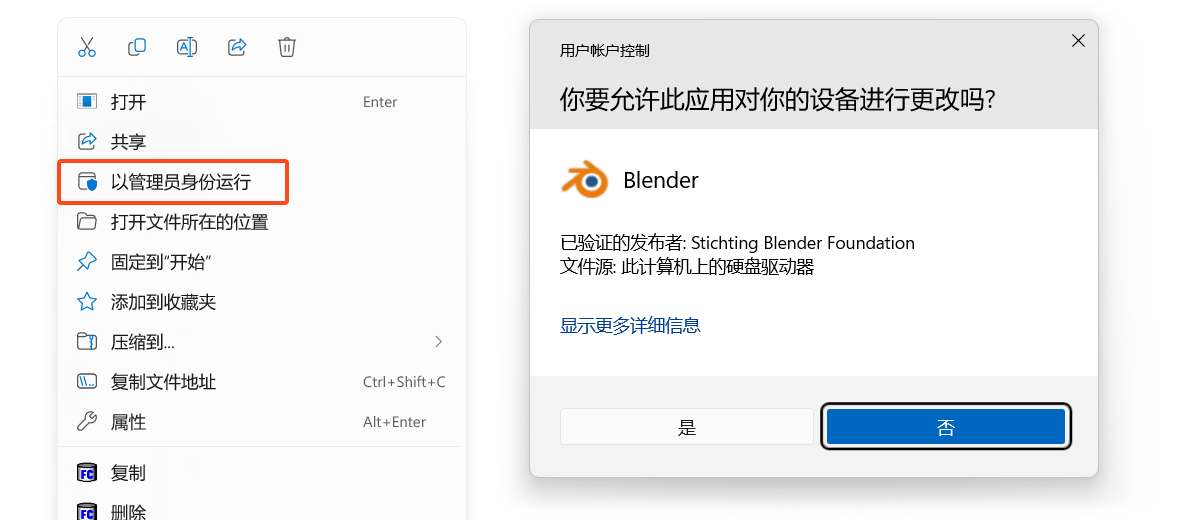
\includegraphics[width=.7\textwidth]{assets/advanced/Menu_and_UAC.png}
  \caption{右键菜单的【以管理员身份运行】与 UAC 弹窗}
  \label{fig:Menu_and_UAC}
\end{figure}

有时,我们会遇到一些程序报错,提示【请联系你的管理员】【请联系 Windows 管理员】等信息。这种说法是多用户时代的遗留——彼时,为防止普通用户不小心破坏电脑的关键部分,供多人使用的电脑上,普通人往往只拥有标准用户,无法提权;而管理员用户则由专人担任。所以,那时的普通用户,若需要安装一些软件,或者需要调整系统的关键设置,就需要线下联系他们来进行。这就是程序提示「请联系管理员」的原因。今天,我们的个人电脑不再是「共享电脑」,而程序所称的「管理员」,就是我们自己。

到此为止,我们都在说「我们可以创建的用户」。但其实系统之中,除了我们创建的用户之外,还存有一个\regcolor{隐藏的「超级用户」}——Administrator(直译是「管理员」)。这个用户和我们创建的管理员不同,它\regcolor{只有一种权限层级——管理员权限}。所以,它无论何时都有非常高的权限:更改系统关键设置、安装/卸载软件、创建新的用户、删除别的用户……甚至还可以「窥探」其他用户的文件。由于 Administrator 的权限太高、法术太强,Windows 系统便把它「封印」起来——它不可见、不可登录,甚至不可感知。而它的作用,一般是在我们自己的用户出现意料之外的故障时,用来救急。

我们将 Windows 中常用的三类用户和两种权限总结为下表:

\begin{table}[htb!]
  \centering
  \caption{用户与权限速查表}
  \label{tab:users-and-permissions}
  \begin{tblr}{
      colspec = cccc,
      row{1} = {valign=m, fg = white, bg = missing, font = \bfseries},
      row{even} = {MissingSkyBlue},
    }
    \toprule
    不同的用户 & 标准用户权限 & 管理员权限 & 备注 \\
    \midrule
    普通用户    & 默认 &   无   & --- \\
    管理员     & 默认 & 可提权 & 一般我们自己使用的用户都是管理员 \\
    Administrator &  无  &  默认  & 隐藏用户,被「封印」,无法直接使用 \\
    \bottomrule
  \end{tblr}
\end{table}

\begin{note}
  在过去盗版、修改版系统横行的年代,许多国内盗版和修改版的 Windows 系统,会强行解除 Administrator 用户的「封印」,并把它作为系统的默认用户。尽管这样,我们将不再见到有些恼人的「UAC 弹窗」(因为此时我们总是以管理员权限运行程序),但这时,我们相当于头上悬着一把「\href{https://baike.baidu.com/item/%E8%BE%BE%E6%91%A9%E5%85%8B%E5%88%A9%E6%96%AF%E4%B9%8B%E5%89%91/231450}{\regcolor{达摩克利斯之剑}}」在系统中四处穿行,其危险性可想而知。
\end{note}

\section{「本地帐户」和微软账号}

你用过手机上的「云服务」吗?近年来,诸如 iCloud、华为云服务、小米账号这样的云服务在一定程度上提升了我们使用手机的便利程度。事实上,微软在 Windows 系统上也有着类似的服务:我们可以将系统中的用户和在线的「微软账号」(称为「Microsoft 帐户」)绑定,实现诸如同步等的各种附加功能。

为了和「已经绑定了微软账号的用户」区分,Windows 专门为传统的用户起了个名字——「本地帐户」。将「本地帐户」链接到微软账号后,微软账号的登录密码就会变成我们开机使用的密码(除此之外还可以设置额外的数字密码),微软账号的用户名就变成了我们\regcolor{显示在屏幕上}的用户名\cprotect\footnote{本地存储的用户名是不会因为绑定到微软账号而改变的。即,绑定前后,打开 \MissingVerb{C:\用户\ } 看到的文件夹名字是一样的。}。

在 Windows 11 上,打开系统设置,转到【帐户】→【帐户信息】,选择【改用 Microsoft 帐户登录】,即可将自己的「本地帐户」和微软账号绑定。

\begin{figure}[htb!]
  \centering
  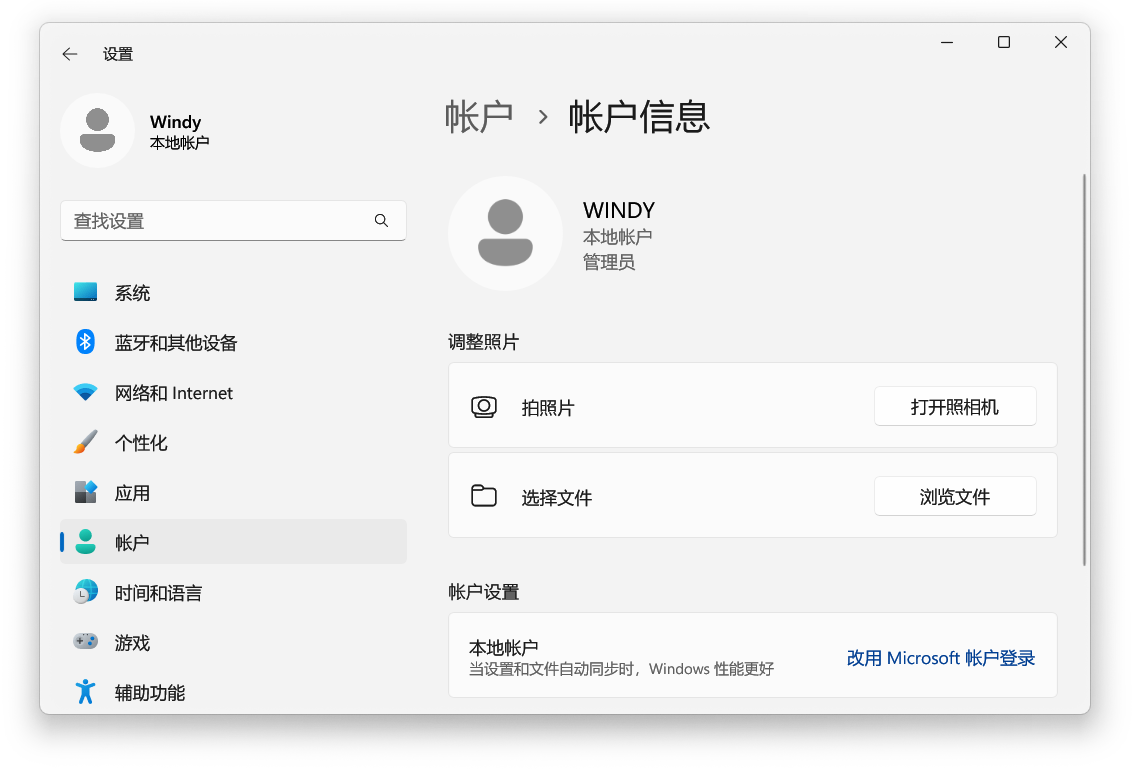
\includegraphics[width=.65\textwidth]{assets/advanced/Login_with_MS_accont_Win11.png}
  \caption{Windows 11 的登录选项}
  \label{fig:Login_with_MS_accont_Win11}
\end{figure}

而在 Windows 10 上,则需打开系统设置 →【帐户】,选择【改用 Microsoft 帐户登录】。

\begin{figure}[htb!]
  \centering
  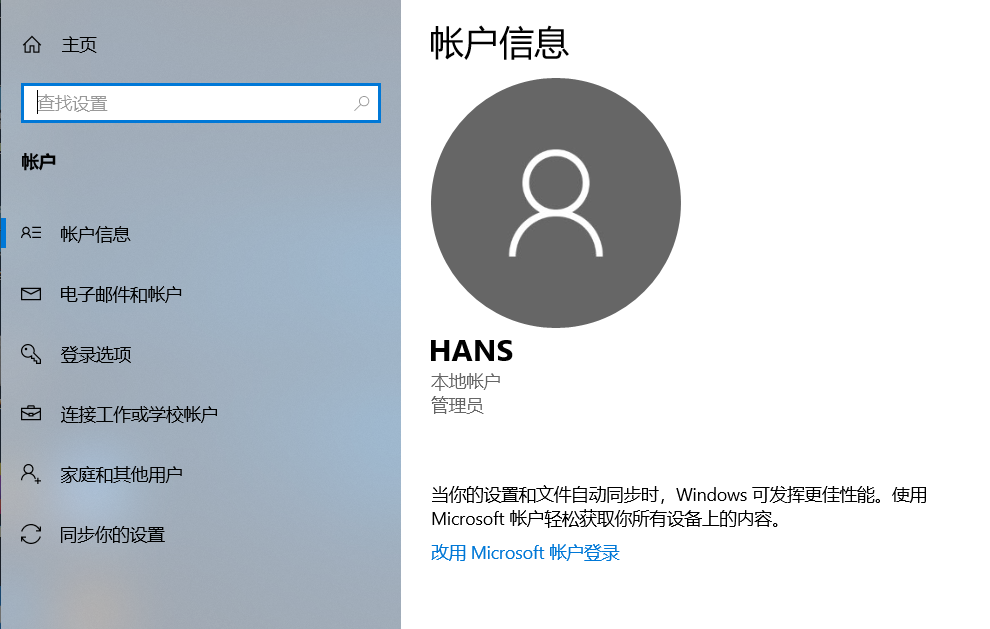
\includegraphics[width=.6\textwidth]{assets/advanced/Login_with_MS_accont_Win10.png}
  \caption{Windows 10 的登录选项}
  \label{fig:Login_with_MS_accont_Win10}
\end{figure}

我们建议读者在自己的电脑上以微软账号登录。将自己的「本地帐户」绑定微软账号有着这些好处:

\begin{itemize}
  \item 更多的用户相关功能,例如 Windows Hello 解锁。
  \item 电脑内的一系列微软自家 app,例如 Microsoft Store 和 Xbox 都将自动登录。
  \item 主题、壁纸和基本设置同步。这意味着,如果你有多台 Windows 电脑,那么设置会在这些设备中同步(可以手动关闭)。
  \item 跨设备剪切板。如果你有多台 Windows 电脑,那么在一台电脑上复制的东西(理论上)可以在另一台电脑粘贴。
  \item \CJKsout*{你甚至可以为你的微软账号设置一个好看的头像,让电脑在开机时赏心悦目一点。}
  \item ……
\end{itemize}

\section{设备加密与微软帐号}

\begin{warning}
  打开【此电脑】,观察你的磁盘图标上是否有挂锁图案。若有,请务必阅读这部分内容。
  
  \begin{center}
    \centering
    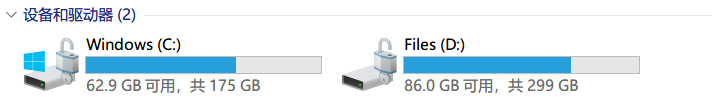
\includegraphics[width=.8\textwidth]{assets/advanced/BitLocker.png}
    \captionof{figure}{设备加密锁}
    \label{fig:BitLocker}
  \end{center}
\end{warning}

如果在【此电脑】中,你看到了带挂锁图案的磁盘图标,说明你的电脑启用了「设备加密」。一些电脑在出厂的时候会启用这个功能。这功能启用后,硬盘上的所有数据都是加密存储的,而那用来解密的,\regcolor{长达 48 个字符}的密钥,存储在电脑内部的一个安全芯片中。这个安全芯片会在电脑开机时检查系统安全情况——例如,开机过程中有无恶意软件作祟,电脑是否有被恶意开启并篡改过设置等。当这个芯片确认安全后,它就会向系统通报密钥并进行解密。整个过程中,用户看不到密钥。

在某些极端情况下,这个芯片可能产生误判。一旦它认为启动环境不安全,就会拦截启动过程,不再向系统通报密钥。这时你将会在开机时卡在这个画面:

\begin{figure}[htb!]
  \centering
  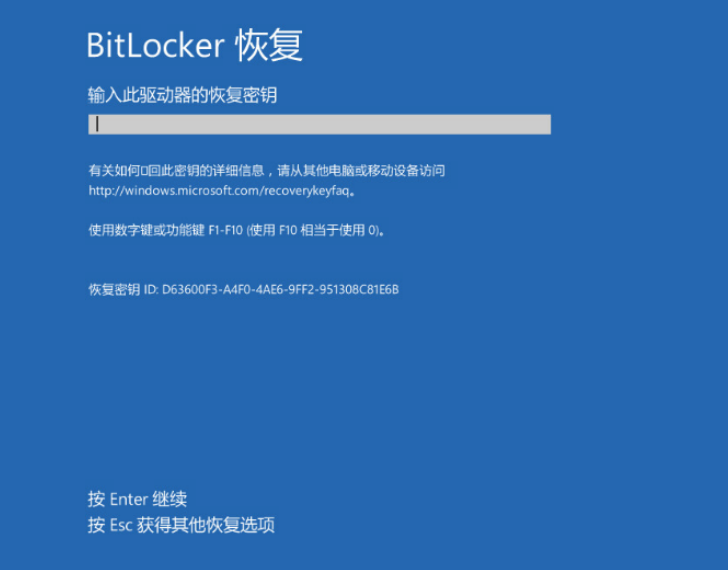
\includegraphics[width=.6\textwidth]{assets/advanced/RecoverPass.png}
  \caption{设备加密恢复界面}
  \label{fig:RecoverPass}
\end{figure}

可是,我们作为普通用户,从来没见过那长长密钥的真面目啊。这时,如果你使用过微软账号来登录系统,那么你不必担心找不到这个密钥,微软会自动帮你把它备份到云端。你只需要打开 \url{https://account.microsoft.com/devices/recoverykey} 这个链接,按提示登录微软账号,即可找到自己设备所有加密分区的,长达 48 字符的密钥。\CJKsout*{虽然但是,谁愿意手打那么长的密钥啊。}

\begin{figure}[htb!]
  \centering
  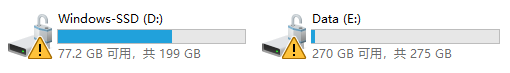
\includegraphics[width=.7\textwidth]{assets/advanced/Bitlocker_Unfinished.png}
  \caption{未完成的设备加密}
  \label{fig:Bitlocker_Unfinished}
\end{figure}

如果你在新机配置时没有登录微软账号,电脑上的设备加密可能会处于「还差最后一块拼图」的状态,此时的磁盘图标会出现上图那样的黄色警告标志。而打开系统设置→【更新和安全】→【设备加密】,则会看到「你需要 Microsoft 帐户才能完成此设备的加密」的警告信息。

\begin{figure}[htb!]
  \centering
  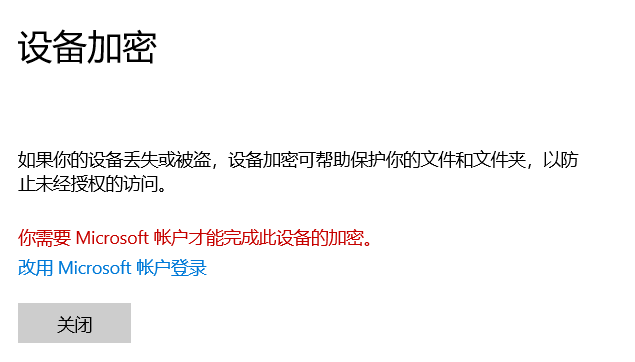
\includegraphics[width=.6\textwidth]{assets/advanced/Bitlocker_Info.png}
  \caption{设备加密的警告信息}
  \label{fig:Bitlocker_Info}
\end{figure}

没错,这「最后一块拼图」就是将「本地帐户」连接到微软账号。但此时,系统有可能已经完成了磁盘的加密工作,也就意味着电脑在使用时依然有概率陷入「输入恢复密钥」的尴尬场面。但因为你的用户未连接微软账号,也就无从查找那「恢复密钥」,而设备加密采用的加密算法非常复杂,从理论上不可能被强行破解,这时我们就只能尝试多次重启、排查造成芯片认为不安全的因素来尝试进入系统了。因此,\regcolor{如果你的电脑启用了设备加密,请务必将「本地帐户」连接到微软账号!}

\begin{note}
  对「加密」与「安全」感兴趣?可以阅读本书超越篇的\chapref{cha:introduction-to-cryptology}。
\end{note}

\section{更改用户文件夹名 *}

众……可能不所周知,部分软件(尤其是国外软件)无法正确处理带有中文等字符的路径,导致当用户名存在中文等字符时无法正常工作。然而,即便你在【控制面板】→【用户帐户】中改掉你的用户名,也不会改变用户建立之初就确定下来的用户文件夹名,此时,我们需要额外的操作来更改用户文件夹名。

\begin{figure}[htb!]
  \centering
  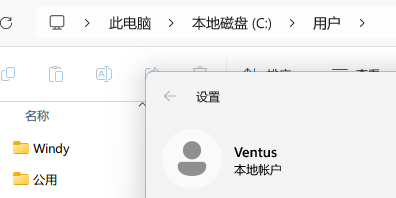
\includegraphics[width=.5\textwidth]{assets/advanced/Unchanged_User_Folder.png}
  \caption{仍是原用户名的文件夹}
  \label{fig:Unchanged_User_Folder}
\end{figure}

上图中,即使用户名被改成了 Ventus,但用户文件夹名仍然是原来的 \MissingVerb{Windy}。接下来,我们将详细演示如何将用户文件夹名也修改成 \MissingVerb{Ventus}。

\begin{danger}
  在着手操作之前,请\regcolor{一定确保电脑上没有在运行或自动运行的任何云存储服务}(包括但不限于 OneDrive、iCloud、百度网盘等)。如果有,请预先停止自动同步或关闭自动启动。
\end{danger}

\subsection{获取当前用户的 SID}

\begin{figure}[htb!]
  \centering
  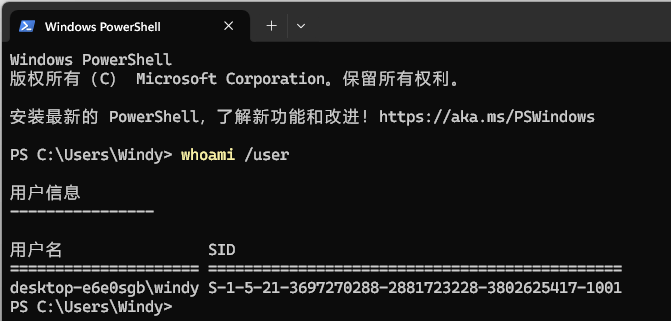
\includegraphics[width=.6\textwidth]{assets/advanced/Get_SID.png}
  \caption{获取 SID}
  \label{fig:Get_SID}
\end{figure}

SID,即「安全标识符」(security identifier),用于在操作系统中唯一地标识安全主体或安全组,包括用户和用户组等。简而言之,SID 就是操作系统给这台电脑上的所有用户派发的「身份证」,靠着这个「身份证」,操作系统才能识别用户、准许用户访问自己的资源。

既然我们想改变自己用户的信息,那么很显然记下当前用户的 SID 是非常有必要的。按下 \keys{\Windows + X},选择【终端】或【PowerShell】,输入 \MissingVerb{whoami /user},回车,即可看到当前用户的 SID。SID 是随机生成的,所以要是看到和\autoref{fig:Get_SID} 一样的,不妨去买张彩票?

\subsection{新建一个临时管理员用户}

为了对现有的用户进行操作,我们需要先创建一个临时的管理员用户,借助它来完成转换。转到设置 →【帐户】→【其他用户】,点击【添加帐户】,在弹出的窗口中依次点击【我没有这个人的登录信息】【同意并继续】【添加一个没有 Microsoft 帐户的用户】,然后随意设置一个用户名(\regcolor{千万不要设置成你希望修改成的用户文件夹名},在本例中是 Ventus),如 Reimu。

\begin{figure}[htb!]
  \centering
  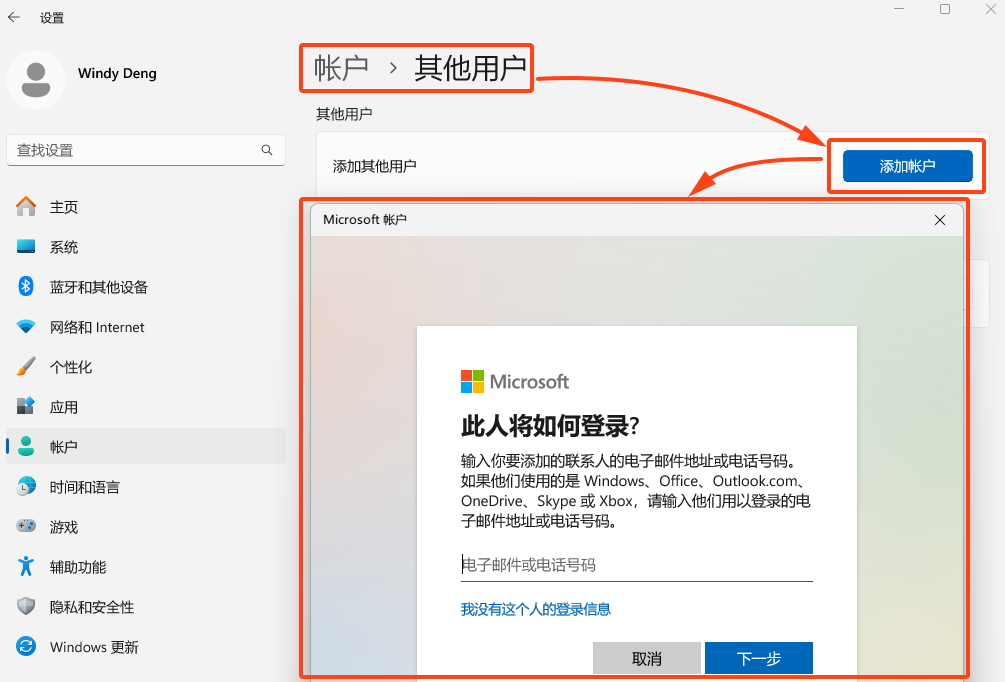
\includegraphics[width=.7\textwidth]{assets/advanced/New_User.png}
  \caption{新建用户}
  \label{fig:New_User}
\end{figure}

默认情形下,新建的用户会是「标准用户」,无法进行提权操作,所以接下来我们要把它改成管理员用户。点击用户列表中刚刚新建的用户,点击【更改帐户类型】,改成「管理员」即可。

\begin{figure}[htb!]
  \centering
  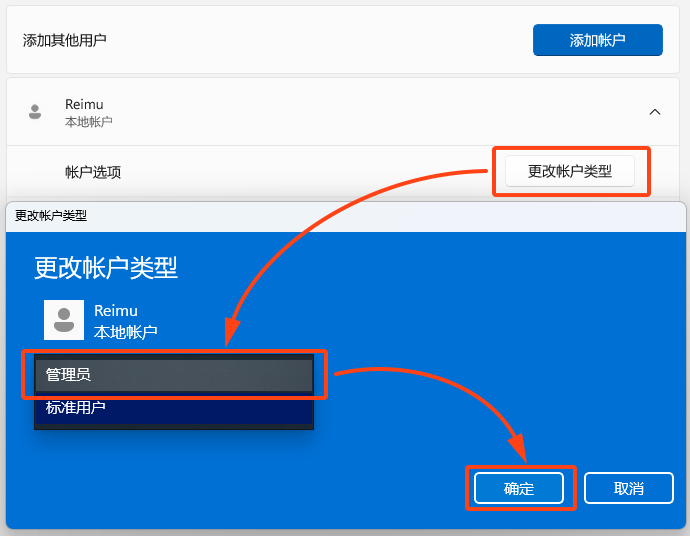
\includegraphics[width=.5\textwidth]{assets/advanced/Change_User_Type.png}
  \caption{更改新用户为管理员}
  \label{fig:Change_User_Type}
\end{figure}

\subsection{在新管理员用户下操作原用户的文件夹}

注销(事实上是登出)当前用户,切换到刚刚创建的临时管理员用户。打开任务管理器,切换到【用户】选项卡,\regcolor{确保那里面只显示当前登录的用户}(本例中是 Reimu),若原来的用户还在,则需要重新登回去,确保注销。

\begin{figure}[htb!]
  \centering
  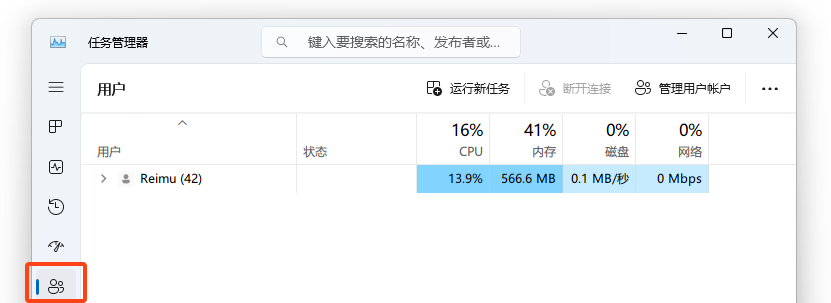
\includegraphics[width=.7\textwidth]{assets/advanced/Users_In_Tskmgr.png}
  \caption{在任务管理器中查看活动用户}
  \label{fig:Users_In_Tskmgr}
\end{figure}

确定只有当前用户后,打开资源管理器,转到 \MissingVerb{C:\用户\} 下,\regcolor{更改原来的用户文件夹名称为你想要的名字},本例中是 \MissingVerb{Ventus}。好,我们有了一大进步!

\begin{figure}[htb!]
  \centering
  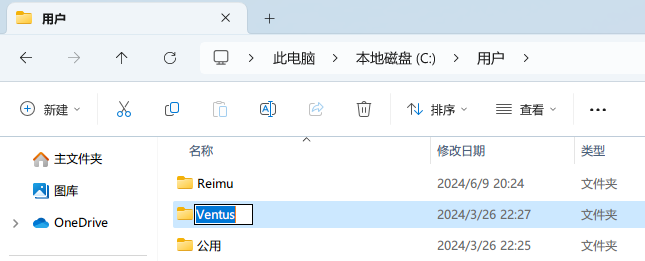
\includegraphics[width=.7\textwidth]{assets/advanced/Change_User_Folder_Name.png}
  \caption{重命名原来的用户文件夹}
  \label{fig:Change_User_Folder_Name}
\end{figure}

\subsection{修改注册表以匹配新名字}

\begin{danger}
  这一步需要非常细心的操作,一定不能出错!
\end{danger}

按下 \keys{\Windows + R},输入 \MissingVerb{regedit},确定,打开注册表编辑器,转到以下地址(你也可以把这一行复制粘贴到注册表编辑器的地址栏去):

\begin{MissingVerbatim}
  HKEY_LOCAL_MACHINE\SOFTWARE\Microsoft\Windows NT\CurrentVersion\ProfileList
\end{MissingVerbatim}

接下来是当初记下的 SID 的用武之地了,在左侧 \MissingVerb{ProfileList} 文件夹下找到第 1 步记下的 SID,点进去,可见右侧 \MissingVerb{ProfileImagePath} 一项正是你原来的用户文件夹路径,\regcolor{先记下来,下一步要用}。将它的尾部你原来用户文件夹名的部分 \MissingVerb{Windy} 改成新文件夹名 \MissingVerb{Ventus} 即可。

\begin{figure}[htb!]
  \centering
  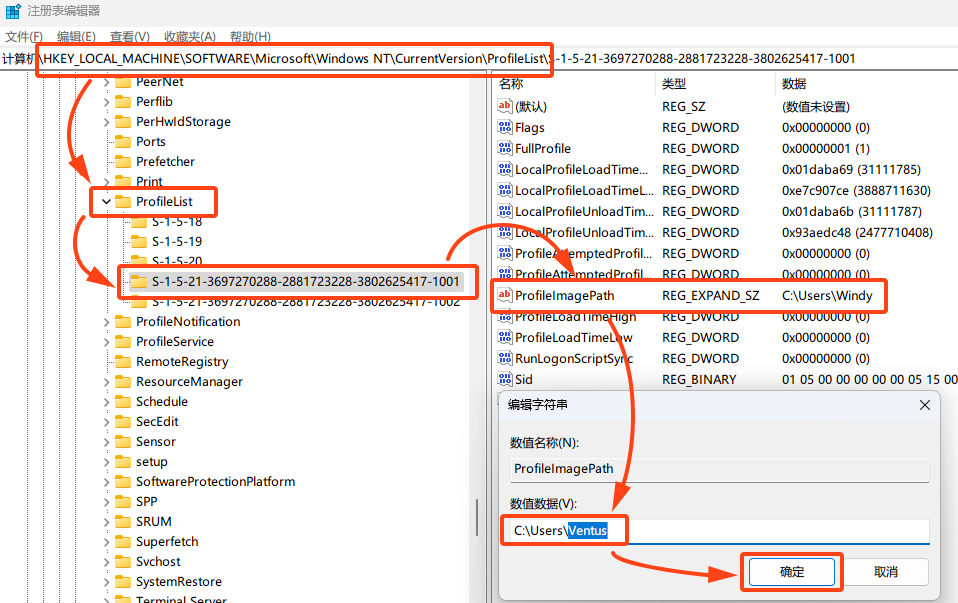
\includegraphics[width=.7\textwidth]{assets/advanced/Change_Reg.png}
  \caption{更改注册表条目}
  \label{fig:Change_Reg}
\end{figure}

\subsection{建立新旧用户文件夹间的符号链接}

\begin{danger}
  这一步也是重中之重,一定不能出错!
\end{danger}

符号链接相当于通用的「快捷方式」,访问符号链接就相当于访问它指向的目标,欲了解更多,可以阅读\chapref{cha:manage-storage}一章。所以,建立符号链接的目的就是让那些已有的软件在照旧访问原来的用户文件夹时能够访问到修改后的位置。

首先按 \keys{\Windows + S},搜索 \MissingVerb{cmd},右击【命令提示符】,选择【以管理员身份运行】,输入
\begin{MissingVerbatim}
  mklink /d <旧用户文件夹路径> <新用户文件夹路径>
\end{MissingVerbatim}
譬如在本节的情形下,就输入
\begin{MissingVerbatim}
  mklink /d C:\Users\Windy C:\Users\Ventus
\end{MissingVerbatim}
回车,你就可以在 \MissingVerb{C:\用户\} 下看到符号链接了。如果它提示「已存在」,那肯定是你忘记重命名了。

\subsection{收尾工作}

至此,我们要做的工作已经尽数完成,可以继续使用原本的用户了。虽然可能有部分软件中仍然显示着曾经的用户文件夹路径,但不必担心,我们不是建立了符号链接吗?脑海中「翻译」一下就好啦。

不过,仍然有一些事情可能需要我们处理。如果你照\chapref{cha:file-and-file-management}中的方法更改了用户文件夹的存储位置,那么,你可能会发现自己的文件不见了,这是因为系统没有为新的用户文件夹路径记录存储位置。虽说文件还在之前改过的存储位置那里放着,但还是需要重新操作一遍更改。至于我们新建的那个临时管理员用户,你可以在设置中将它删除。

\CJKsout*{以及,你没法建立一个与原用户相同名称的新用户了。}

\practice

\begin{enumerate}
  \item 查看自己的用户名,检查自己是以「本地帐户」登录的还是以微软账号登录的。
  \item 检查自己的设备是否有启用设备加密。一般来说,只有部分品牌系列的「商务本」才会默认启用这个功能。
  \item 为什么说将 Administrator 作为主用户登录无异于悬着一把「达摩克利斯之剑」?
\end{enumerate}